\section{Experiments}
\input{Tables/combined_table}
In this section, we systematically validate the effectiveness of the proposed \emph{Language-Aware Skeleton Exploration Framework (\Lasef)} across diverse settings. The experiments are designed to analyze performance by varying model scale, problem difficulty, and language resource levels, while keeping the structure and generation method of the skeleton fixed. Through this, we analyze (1) whether the effectiveness of skeleton-based reasoning is limited to specific conditions, and (2) how it varies according to language and model characteristics.

\subsection{Experimental Setup}
% \paragraph{Models based on Scale.} To analyze how the effect of skeletons varies with model scale, following the approach of Structure-of-Thought~\citep{qi2025sot}, we selected the \textsc{Qwen2.5}~\citep{qwen2025qwen25technicalreport} series as our base models, which are general-purpose models known for superior multilingual capabilities rather than being specialized solely for reasoning. Specifically, we used three different model sizes—Qwen2.5-7B, 14B, and 72B—to analyze how the impact of skeleton-based structural guidance changes as model scale increases. We also conducted experiments with the \textsc{Llama~3.1} series~\citep{grattafiori2024llama3herdmodels}, which are reported in Appendix~\ref{Appendix:Llama-results}.

\paragraph{Models based on Scale.} 
To analyze the impact of model scale, we select the \textsc{Qwen2.5} series~\citep{qwen2025qwen25technicalreport} as our base models, following prior research~\citep{qi2025sot}. These models are chosen for their superior multilingual capabilities as general-purpose models, rather than being specialized solely for reasoning. We utilize three distinct sizes (7B, 14B, 72B) to examine how the efficacy of skeleton guidance evolves with scale. For brevity, we refer to the \textsc{Qwen2.5-Instruct} models simply by their sizes (e.g., \textsc{Qwen2.5-14B}). Results for the \textsc{Llama~3.1} series~\citep{grattafiori2024llama3herdmodels} are provided in Appendix~\ref{Appendix:Llama-results}.

% \paragraph{Benchmarks based on Difficulty Levels.} To examine the impact of skeletons by problem difficulty, we organized mathematical reasoning benchmarks by difficulty level. We used MGSM~\citep{shi2022language} to evaluate elementary-level multilingual arithmetic reasoning, and MATH-500~\citep{lightman2023let} to include intermediate-level systematic mathematical problems. Finally, we employed PolyMath~\citep{wang2025polymath}, which requires advanced complex reasoning capabilities, to analyze how the effectiveness of skeletons changes as the problem structure becomes more complex.
\paragraph{Benchmarks by Difficulty.} 
We categorize our benchmarks by difficulty to assess skeleton effectiveness across task complexities. We employ MGSM~\citep{shi2022language} for elementary arithmetic, MATH-500~\citep{lightman2023let} for intermediate-level problems, and PolyMath~\citep{wang2025polymath} for advanced reasoning tasks requiring complex structural analysis.

\paragraph{Target Languages based on Resource Levels.} To evaluate the impact of skeletons according to language resource levels, we included diverse target languages, from high-resource to low-resource. High-resource languages were selected based on their sufficient exposure during large-scale pre-training, while low-resource languages were chosen based on the relative scarcity of training data, which often leads to inconsistent reasoning performance in multilingual LLMs. This allows us to analyze whether skeletons play different roles depending on the resource level of the language.

% \paragraph{Evaluation Protocol.} All experiments utilized greedy decoding to minimize variability in the reasoning process. Quantitative evaluation was conducted using the \texttt{math-verify} library~\citep{mathverify}, measuring Exact Match (EM) based on whether the model's output strictly matches the ground truth. To ensure a fair comparison of reasoning capabilities, we only evaluated samples where the output language remained consistent. Specifically, we included only those samples satisfying the condition $\ell_a=\ell_t$, where the answer is generated in the target language, thereby preventing evaluation distortion due to language mixing or code-switching. Further details on the evaluation methodology are described in Appendix~\ref{Appendix:Evaluation-protocol}.
\paragraph{Evaluation Protocol.} 
We evaluate performance based on Exact Match (EM). Crucially, to ensure the validity of multilingual reasoning, we strictly restrict our evaluation to samples satisfying the condition $\ell_a=\ell_t$, where the generated answer language matches the target language. Further details on the experimental setup are provided in Appendix~\ref{Appendix:Evaluation-setup}.



\subsection{Baseline Configurations}
% To analyze the effectiveness of \LASEF, we explicitly define the language combination $(\ell_q, \ell_s, \ell_a)$—corresponding to the query, skeleton, and reasoning/answer languages—for a given target language $\ell_t$, and establish an appropriate comparative baseline. 
To analyze the effectiveness of \Lasef, we define the language combination $(\ell_q, \ell_s, \ell_a)$ for a given target language $\ell_t$, and establish an appropriate comparative baseline. Since skeletons function as structural guides for improving reasoning performance, we adopt a Chain-of-Thought (CoT)-based setting as the primary baseline~\citep{cot-neurips2022}, following prior work on multilingual reasoning~\citep{xlt-emnlp2023,clp-emnlp2023}.

% CoT generally provides more stable reasoning performance than unstructured prompting, making it a suitable reference point for evaluating the contribution of skeletons[].

\paragraph{Target-Language CoT (\textsc{CoT-$\ell_t$}).} In this setting, the input query is given in the target language, and both reasoning and the answer are generated in the same language $(\ell_q=\ell_a=\ell_t)$. We use a standard CoT prompt (``Let’s think step by step, Respond in {$\ell_t$}'') without applying a skeleton. This represents the most natural usage scenario where users verify both the query and the reasoning process in their native language.

\paragraph{English-Pivot CoT (\textsc{CoT-$en$}).} In this setting, the input query is translated into English $(\ell_q=\text{en})$, after which the reasoning and answer are generated in the target language $\ell_t$. This baseline is essential for two reasons. First, comparing performance based on English-translated queries is a widely used practice in existing multilingual reasoning studies~\citep{clp-emnlp2023,xlt-emnlp2023,trans-allneed-2025naacl}, serving as a benchmark representing the upper-bound performance of LLMs pre-trained primarily on English. Second, even in real-world non-English user environments, since users already understand the meaning of the query, internally converting the query to English does not significantly hinder meaning transmission. Thus, \textsc{CoT-$en$} serves as a rational baseline to evaluate whether performance gains via translation are achievable without structural guidance.

\paragraph{Skeleton Baseline Language Configuration.} 
English skeletons are used in Tab.~\ref{tab:combined-main-table} and \ref{tab:low-resource-mgsm}, while Fig.~\ref{fig:cross-lingual-skeleton} expands to Chinese, Spanish, Russian, Korean, and Thai.

\subsection{Performance across Diverse Dimensions}
Tab.~\ref{tab:combined-main-table} compares \LASEF in an English skeleton setting $(\ell_q, en, \ell_a)$ against baselines across three benchmarks: MGSM, MATH-500, and PolyMath.

% Experimental results indicate that the introduction of English skeletons yields varying effects depending on model size, benchmark difficulty, and language resource levels. Performance gains are more pronounced when (1) the model is smaller, (2) the problem difficulty is lower, and (3) the language is low-resource. For example, with Qwen2.5-7B-Instruct, performance on the MGSM benchmark for Swahili (sw) improves from 63.1 to 71.7 (+8.6) under the \textsc{CoT-$en^{\dagger}$} setting, whereas larger models such as Qwen2.5-72B-Instruct exhibit only marginal gains (+1.2) or stagnation, as observed for Qwen2.5-14B-Instruct. This indicates that skeleton-based methods do not guarantee uniform benefits, but instead exhibit condition-dependent variability.

% Meanwhile, the \textsc{CoT-$en^{\dagger}$} setting—where the query is translated into English for reasoning—consistently outperforms direct reasoning in the target language (\textsc{CoT-$\ell_t$}), reaffirming the strong English prior of language models trained on large-scale data. In the MGSM experiment with Qwen2.5-7B, \textsc{CoT-$en^{\dagger}$} achieves an average score of 76.5, substantially exceeding the 65.3 of \textsc{CoT-$\ell_t$}. This shows that translation alone can yield substantial gains, underscoring its role as a critical baseline for validating the utility of skeleton-based methods.

\paragraph{Bridging the Resource Gap}
% The differences across language resource levels are particularly pronounced. English skeletons yield substantially larger gains for low-resource languages such as \textsc{Swahili (sw)} than for high-resource languages like \textsc{Chinese (zh)} and \textsc{Spanish (es)}. For Qwen2.5-7B-Instruct under the CoT-$en^{\dagger}$ setting on MGSM, Swahili performance improves from 63.1 to 71.7 (+8.6) with the application of English skeletons, whereas Chinese and Spanish show only marginal gains of +0.0 and +1.6, respectively. This pattern is consistently observed across other model scales and benchmarks. For instance, under the CoT-$en^{\dagger}$ setting on MATH-500 with Qwen2.5-72B-Instruct, the average performance increases modestly from 61.5 to 62.4 (+0.9), with the largest gain again occurring for Swahili (+3.7).

% These results suggest that when low-resource languages alone are insufficient to reliably support complex reasoning processes, generating skeletons in a language with stronger reasoning capacity such as English helps stabilize and scaffold the reasoning process.
Language resource levels significantly influence the impact of English skeletons. Gains are substantially larger for low-resource languages like Swahili~(sw) compared to high-resource languages like Chinese~(zh) and Spanish~(es). For instance, with \textsc{Qwen2.5-7B} on MGSM (CoT-$en^{\dagger}$), Swahili performance rose from 63.1 to 71.7 (+8.6), while Chinese and Spanish showed marginal gains (+0.0 and +1.6). This trend persists across scales; with \textsc{Qwen2.5-72B} on MATH-500, Swahili again saw the highest improvement (+3.7). These results indicate that when low-resource languages lack sufficient reasoning stability, English skeletons serve as an essential scaffold to stabilize the process.


\paragraph{Does Scaling Always Guarantee Improvement?}
% \paragraph{Scale-Dependent Effectiveness}
With respect to model scale, we observe that smaller models benefit more from English skeletons, while the effect diminishes or even becomes negative as model size increases. \textsc{Qwen2.5-7B} and \textsc{14B} exhibit performance improvements after applying skeletons across all benchmarks (+0.9 to 2.5). In contrast, \textsc{Qwen2.5-72B} shows an average performance drop of 0.2 after skeleton application under the \textsc{CoT}-$\ell_t$ setting on MGSM and the \textsc{CoT}-$en^{\dagger}$ setting on PolyMath. This suggests that for large-scale models, externally imposed English skeletons may act as an unnecessary constraint rather than a helpful inductive bias.

\paragraph{Does Benchmark Difficulty Limit the Gains?}
% \paragraph{Diminishing Returns at Larger Scales}
Examining performance variations across benchmark difficulty levels, we observe that the contribution of skeletons is larger for easier benchmarks. Using \textsc{Qwen2.5-7B} as the reference model, skeletons yield a performance gain of +2.2 on MGSM, the easiest benchmark, compared to +1.8 on MATH-500, which has medium difficulty, and +1.2 on PolyMath, the most challenging benchmark. This trend suggests that as problem difficulty increases, simple skeleton generation alone becomes insufficient, as harder problems require more sophisticated and precise computational reasoning beyond what skeletons can provide.

\paragraph{Summary of Results.}
% \paragraph{Overall.}
Results show that English skeletons' benefits depend on model scale, task difficulty, and language resources. Gains are most pronounced for smaller models, easier tasks, and low-resource languages. Notably, the CoT-\textsc{$en^{\dagger}$} setting consistently outperforms CoT\textsc{-$\ell_t$}, reaffirming the strong English prior of LLMs. This underscores translation as a critical baseline for validating the incremental utility of skeletons.

\subsection{Robustness of English Skeletons in Low-Resource Languages}
\begin{table}[!t]
\centering
\resizebox{\columnwidth}{!}{
\begin{tabular}{lrrrr}
\toprule
\multirow{2}{*}{\textbf{Language}} &
\multicolumn{2}{c}{\textbf{$\ell_t,en,\ell_t$}} &
\multicolumn{2}{c}{\textbf{$en^{\dagger},en,\ell_t$}}\\
\cmidrule(lr){2-3}\cmidrule(lr){4-5}
 & \textsc{CoT-$l_t$} & +\textsc{Skeleton} & \textsc{CoT-$en^{\dagger}$} & +\textsc{Skeleton} \\
\midrule
\rowcolor{gray!10}\multicolumn{5}{c}{\textbf{\textit{Qwen2.5-7B-Instruct}}}\\
\midrule
kk & 40.08 & 51.42 (\textcolor{red}{+11.34}) & 62.82 & 72.22 (\textcolor{red}{+9.40}) \\
ky & 33.33 & 37.86 (\textcolor{red}{+4.53}) & 61.92 & 65.69 (\textcolor{red}{+3.77}) \\
mn & 27.16 & 33.33 (\textcolor{red}{+6.17}) & 66.96 & 64.78 (\textcolor{blue}{-2.18}) \\
ug & 27.13 & 37.65 (\textcolor{red}{+10.52}) & 57.14 & 60.37 (\textcolor{red}{+3.23}) \\
hy & 50.81 & 56.05 (\textcolor{red}{+5.24}) & 64.49 & 73.88 (\textcolor{red}{+9.39}) \\
lo & 25.51 & 23.48 (\textcolor{blue}{-2.03}) & 48.54 & 48.95 (\textcolor{red}{+0.41}) \\
eu & 20.76 & 19.92 (\textcolor{blue}{-0.84}) & 65.62 & 74.55 (\textcolor{red}{+8.93}) \\
mt & 25.65 & 20.00 (\textcolor{blue}{-5.65}) & 62.11 & 58.59 (\textcolor{blue}{-3.52}) \\
am & 8.23  & 10.29 (\textcolor{red}{+2.06})  & 39.63 & 32.93 (\textcolor{blue}{-6.70}) \\
ne & 54.29 & 52.65 (\textcolor{blue}{-1.64}) & 74.58 & 78.81 (\textcolor{red}{+4.23}) \\
si & 10.16 & 12.20 (\textcolor{red}{+2.04})  & 37.14 & 35.92 (\textcolor{blue}{-1.22}) \\
ps & 26.46 & 26.91 (\textcolor{red}{+0.45}) & 37.62 & 47.03 (\textcolor{red}{+9.41}) \\
sd & 20.27 & 22.07 (\textcolor{red}{+1.80}) & 64.81 & 68.52 (\textcolor{red}{+3.71}) \\
pa & 51.41 & 52.21 (\textcolor{red}{+0.80}) & 55.87 & 52.63 (\textcolor{blue}{-3.24}) \\
gu & 44.35 & 47.98 (\textcolor{red}{+3.63}) & 59.84 & 60.64 (\textcolor{red}{+0.80}) \\
mr & 45.34 & 46.96 (\textcolor{red}{+1.62}) & 75.41 & 74.18 (\textcolor{blue}{-1.23}) \\
or & 44.35 & 43.95 (\textcolor{blue}{-0.40}) & 36.84 & 38.06 (\textcolor{red}{+1.22}) \\
ta & 47.79 & 49.80 (\textcolor{red}{+2.01}) & 69.48 & 69.08 (\textcolor{blue}{-0.40}) \\
ml & 42.74 & 46.37 (\textcolor{red}{+3.63}) & 62.25 & 64.66 (\textcolor{red}{+2.41}) \\
\midrule
\textbf{AVG.}
 & 33.99 & 36.37 (\textcolor{red}{+2.38})
 & 58.06 & 60.08 (\textcolor{red}{+2.02}) \\
\bottomrule
\end{tabular}
}
\caption{\small Performance comparison on 19 low-resource languages (MGSM) using \textsc{Qwen2.5-7B} with English Skeleton. CoT-$en^{\dagger}$: English-translated queries via Google Translate. Parentheses show $\Delta$ gains.}
\label{tab:low-resource-mgsm}
    \vspace{-0.15in}
\end{table}

% Our preceding analysis confirms that the benefits of English skeletons are most pronounced for smaller models, easier benchmarks, and low-resource language conditions. 
Previous analysis confirms that English skeletons are most effective for smaller models, easier benchmarks, and low-resource languages. In this section, we validate this finding by evaluating \textsc{Qwen2.5-7B} on 19 low-resource MGSM languages. This section examines the consistency of skeleton-based CoT improvements under these conditions. The criteria for language selection and our translation methodology are detailed in Appendix~\ref{appendix:mgsm-translation}.

% benchmark using \textsc{Qwen2.5-7B}. The analysis set includes languages with extremely low proportions in the training data, such as Uyghur~(ug), Kyrgyz~(ky), and Kazakh~(kk). Under these conditions, we closely examine whether skeleton-based CoT yields consistent performance improvements. We describe the criteria for selecting low-resource languages in Appendix~\ref{appendix:mgsm-translation}.

Tab.~\ref{tab:low-resource-mgsm} summarizes the performance changes under the target-language input~($\ell_t$) and English-translated input~($en^{\dagger}$) settings. The results show that English skeletons yield robust performance improvements across low-resource language conditions. Specifically, applying skeletons leads to an average improvement of +2.38 in the CoT-$\ell_t$ setting and +2.02 in the CoT-$en^{\dagger}$.

First, under the Native Input~(CoT-$\ell_t$) setting, skeletons substantially unlock the model’s latent reasoning capacity for certain languages, such as Kazakh~(kk) (+11.34) and Uyghur~(ug) (+10.52). However, there also exist cases where performance degrades, such as Maltese~(mt) (−5.65), indicating a high variance in language-specific effects.

Second, under the (CoT-$en^{\dagger}$) setting, the effect of English skeletons becomes considerably more stable. Notably, query translation alone leads to a dramatic increase in average performance, from 33.99 to 58.06
% , highlighting the effectiveness of providing queries in English in low-resource language settings. 
When English skeletons are incorporated, an additional performance gain of +2.02 is observed. In particular, languages such as Armenian~(hy)~(+9.39), Basque~(eu)~(+8.93), and Pashto (ps)~(+9.41) exhibit substantial improvements when structure in the form of skeletons is added on top of translated queries.

% Overall, in low-resource language settings, the model's potential is maximized by synergizing query translation is combined with English skeletons, which jointly mitigate linguistic barriers and structure the reasoning process. 
Overall, in low-resource language settings, the model's potential is maximized when query translation is combined with English skeletons, jointly mitigating linguistic barriers and structuring the reasoning process. This suggests that skeleton-based CoT can serve as an effective reasoning aid even in extremely low-resource language scenarios.


\subsection{Is English the Only Solution for Low-Resource Languages?}
\label{sec:low-resource-nonen}
In the preceding section, we established that English skeletons generally serve as effective reasoning aids. However, a closer examination of the \textsc{CoT-$\ell_t$} results in Tab.~\ref{tab:low-resource-mgsm} reveals that English is not a universal solution for all low-resource languages. Specifically, among the 19 low-resource languages, five languages (lo, eu, mt, ne, or) show performance degradation when English skeletons are applied.

In this section, we extend the proposed \LASEF to a broader set of languages to demonstrate that skeleton language selection cannot be governed by a fixed rule. Instead, we systematically analyze how its effectiveness varies depending on the characteristics of the target language.

% \begin{figure}[!ht]
%     \centering
%     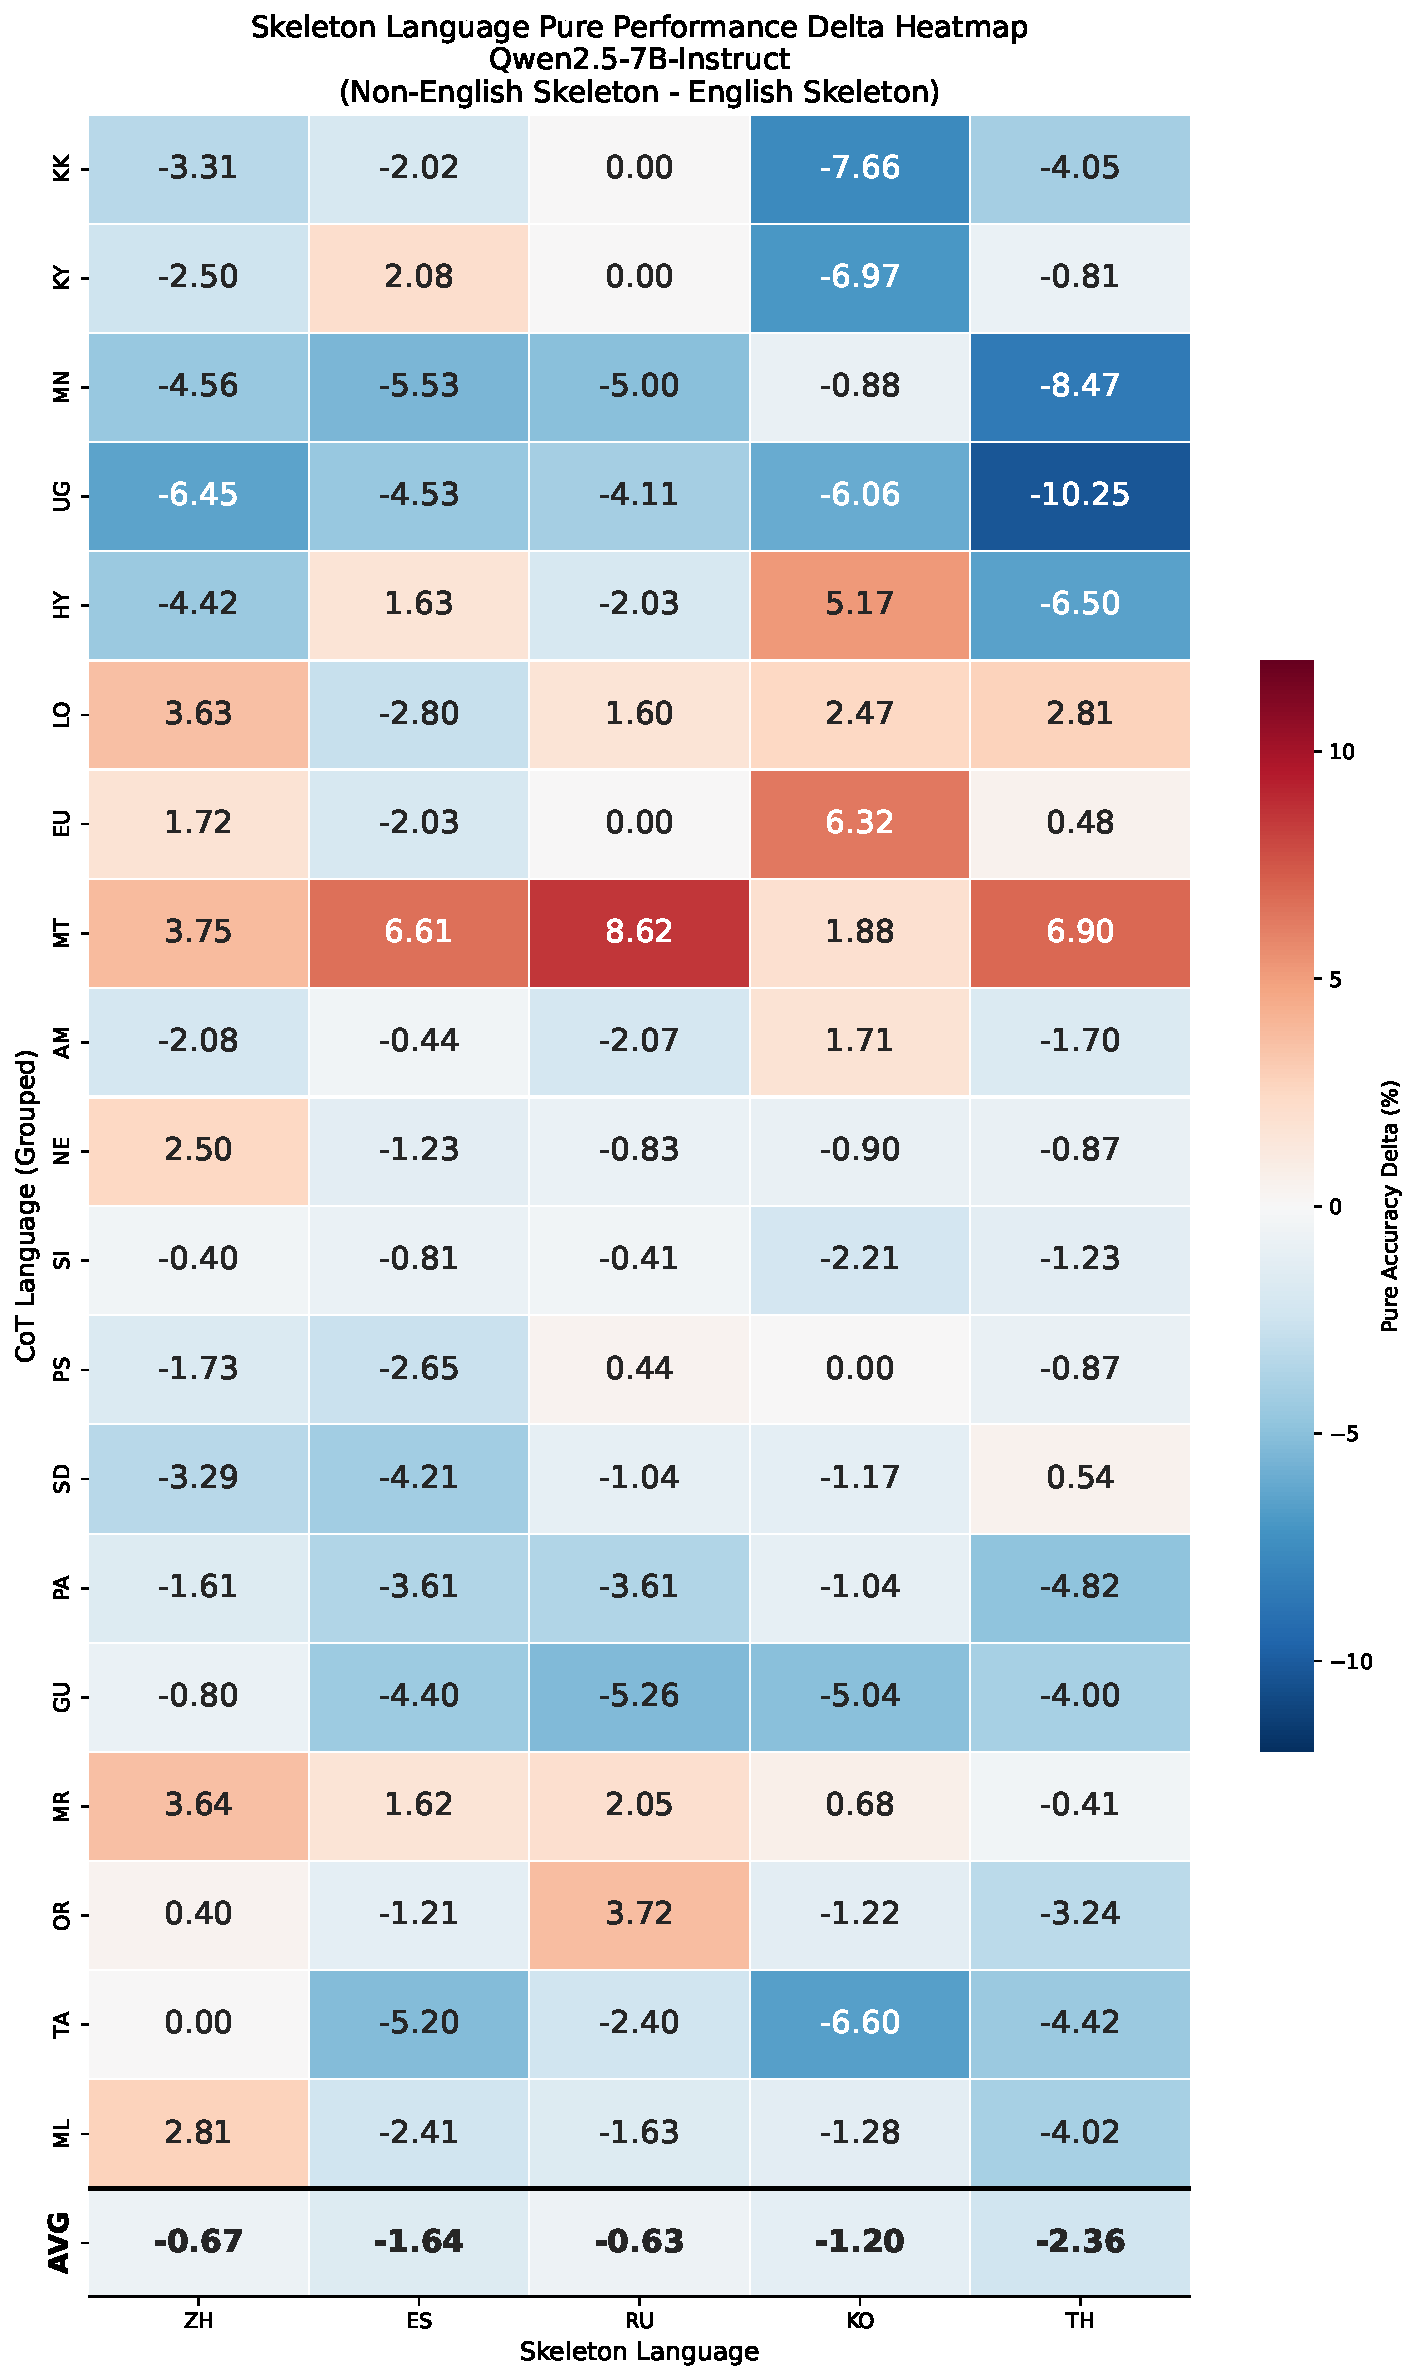
\includegraphics[width=\linewidth]{Figures/Images/Qwen2.5-7B-Instruct_single_pure_delta_heatmap_sorted.pdf}
%     \caption{\small Performance differences (Non-English $-$ English) on the MGSM under the CoT-$\ell_t$ setting with \textsc{Qwen2.5-7B}. English skeleton is replaced with five Non-English skeletons (ZH, ES, RU, KO, and TH). While English generally provides a stable default skeleton language, several target languages exhibit gains with specific Non-English skeletons, indicating that skeleton effectiveness is language-dependent.}
%     \label{fig:cross-lingual-skeleton}
%     \vspace{-0.15in}
% \end{figure}

\begin{figure*}[!ht]
    \centering
    \captionsetup[subfigure]{labelformat=simple, labelsep=space}
    \renewcommand\thesubfigure{(\alph{subfigure})}
    \begin{subfigure}[t]{0.48\linewidth}
        \centering
        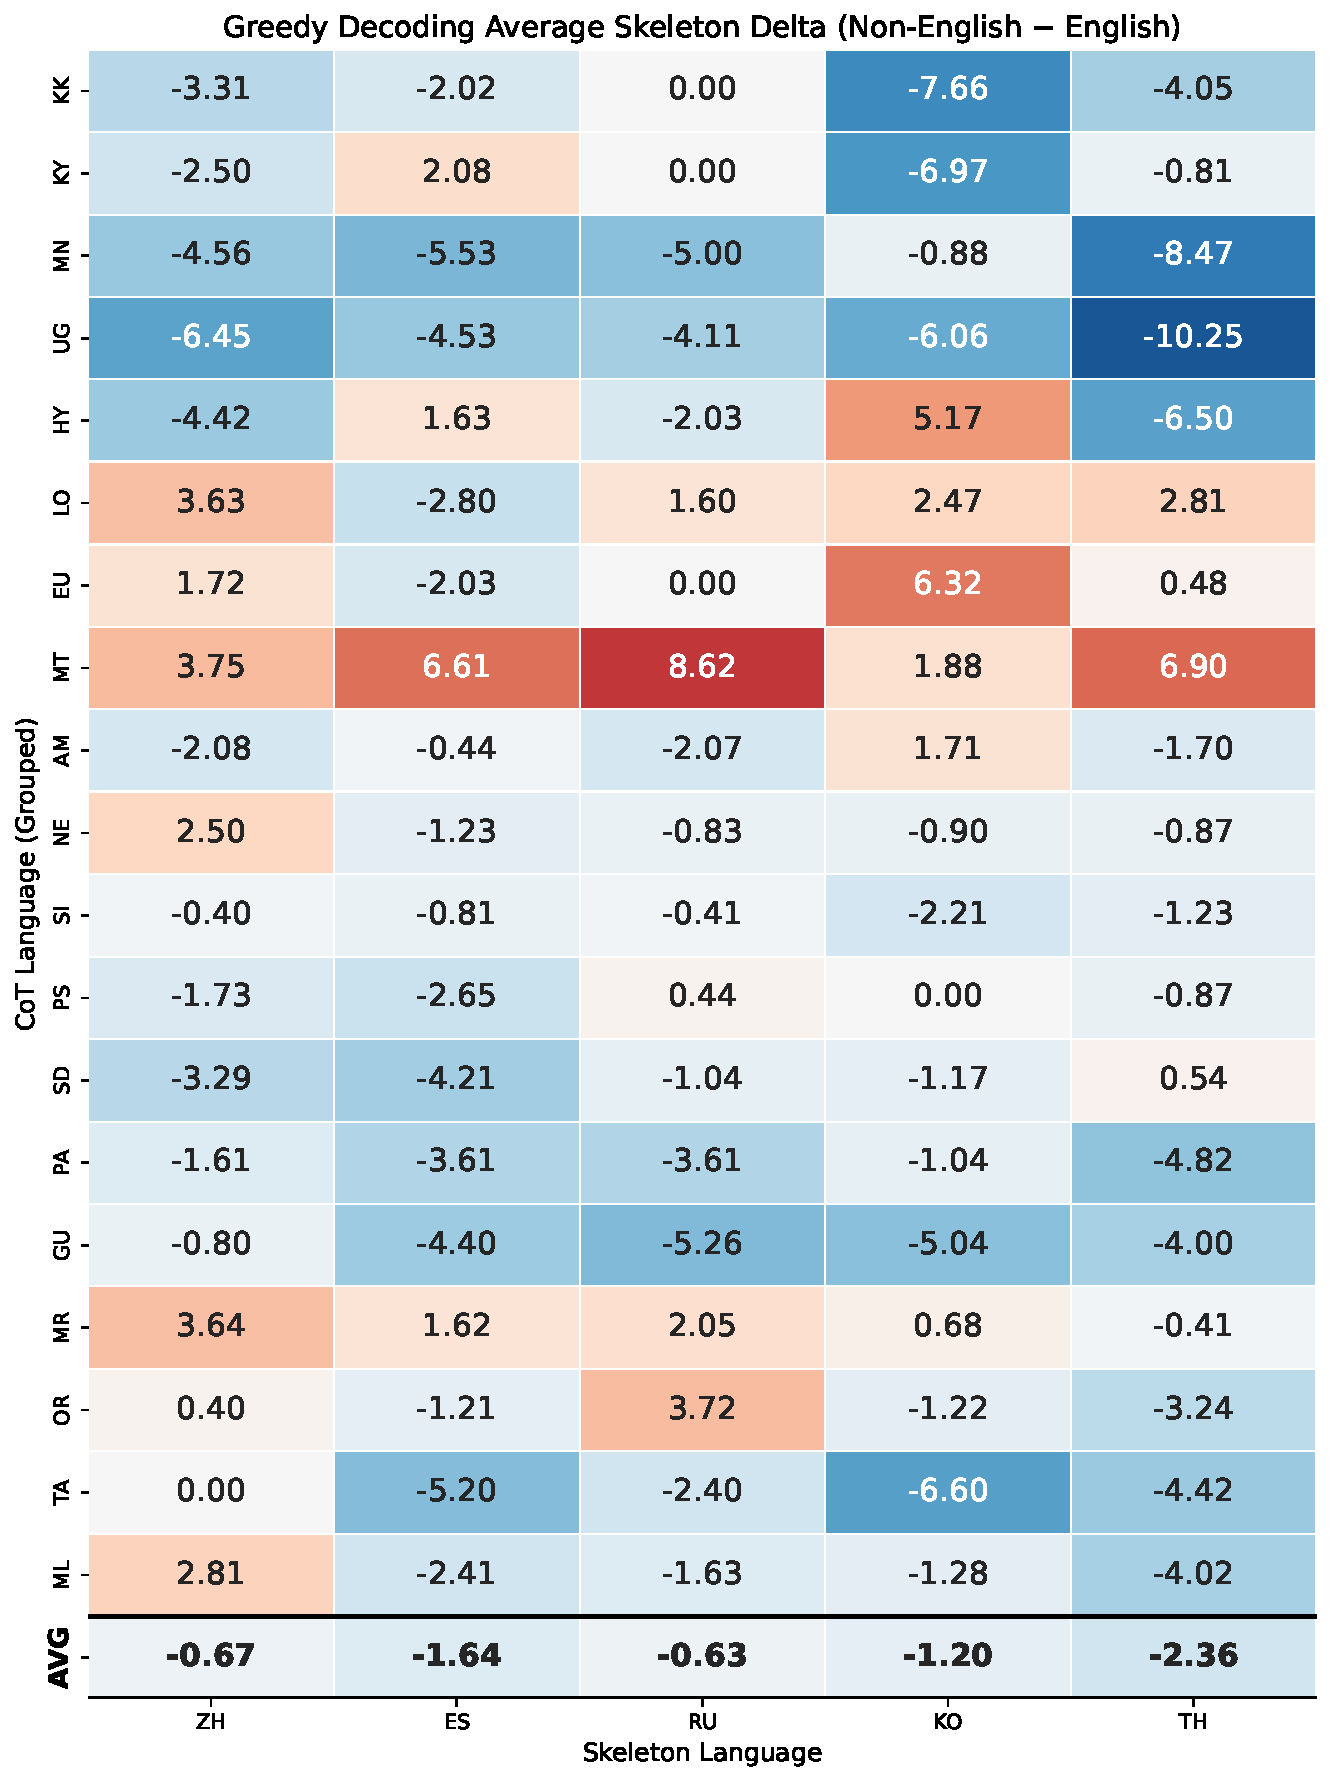
\includegraphics[width=\linewidth]{Figures/Images/greedy.pdf}
        \caption{Greedy Decoding (single rollout)}
        \label{fig:heatmap-greedy}
    \end{subfigure}
    \hfill
    \begin{subfigure}[t]{0.48\linewidth}
        \centering
        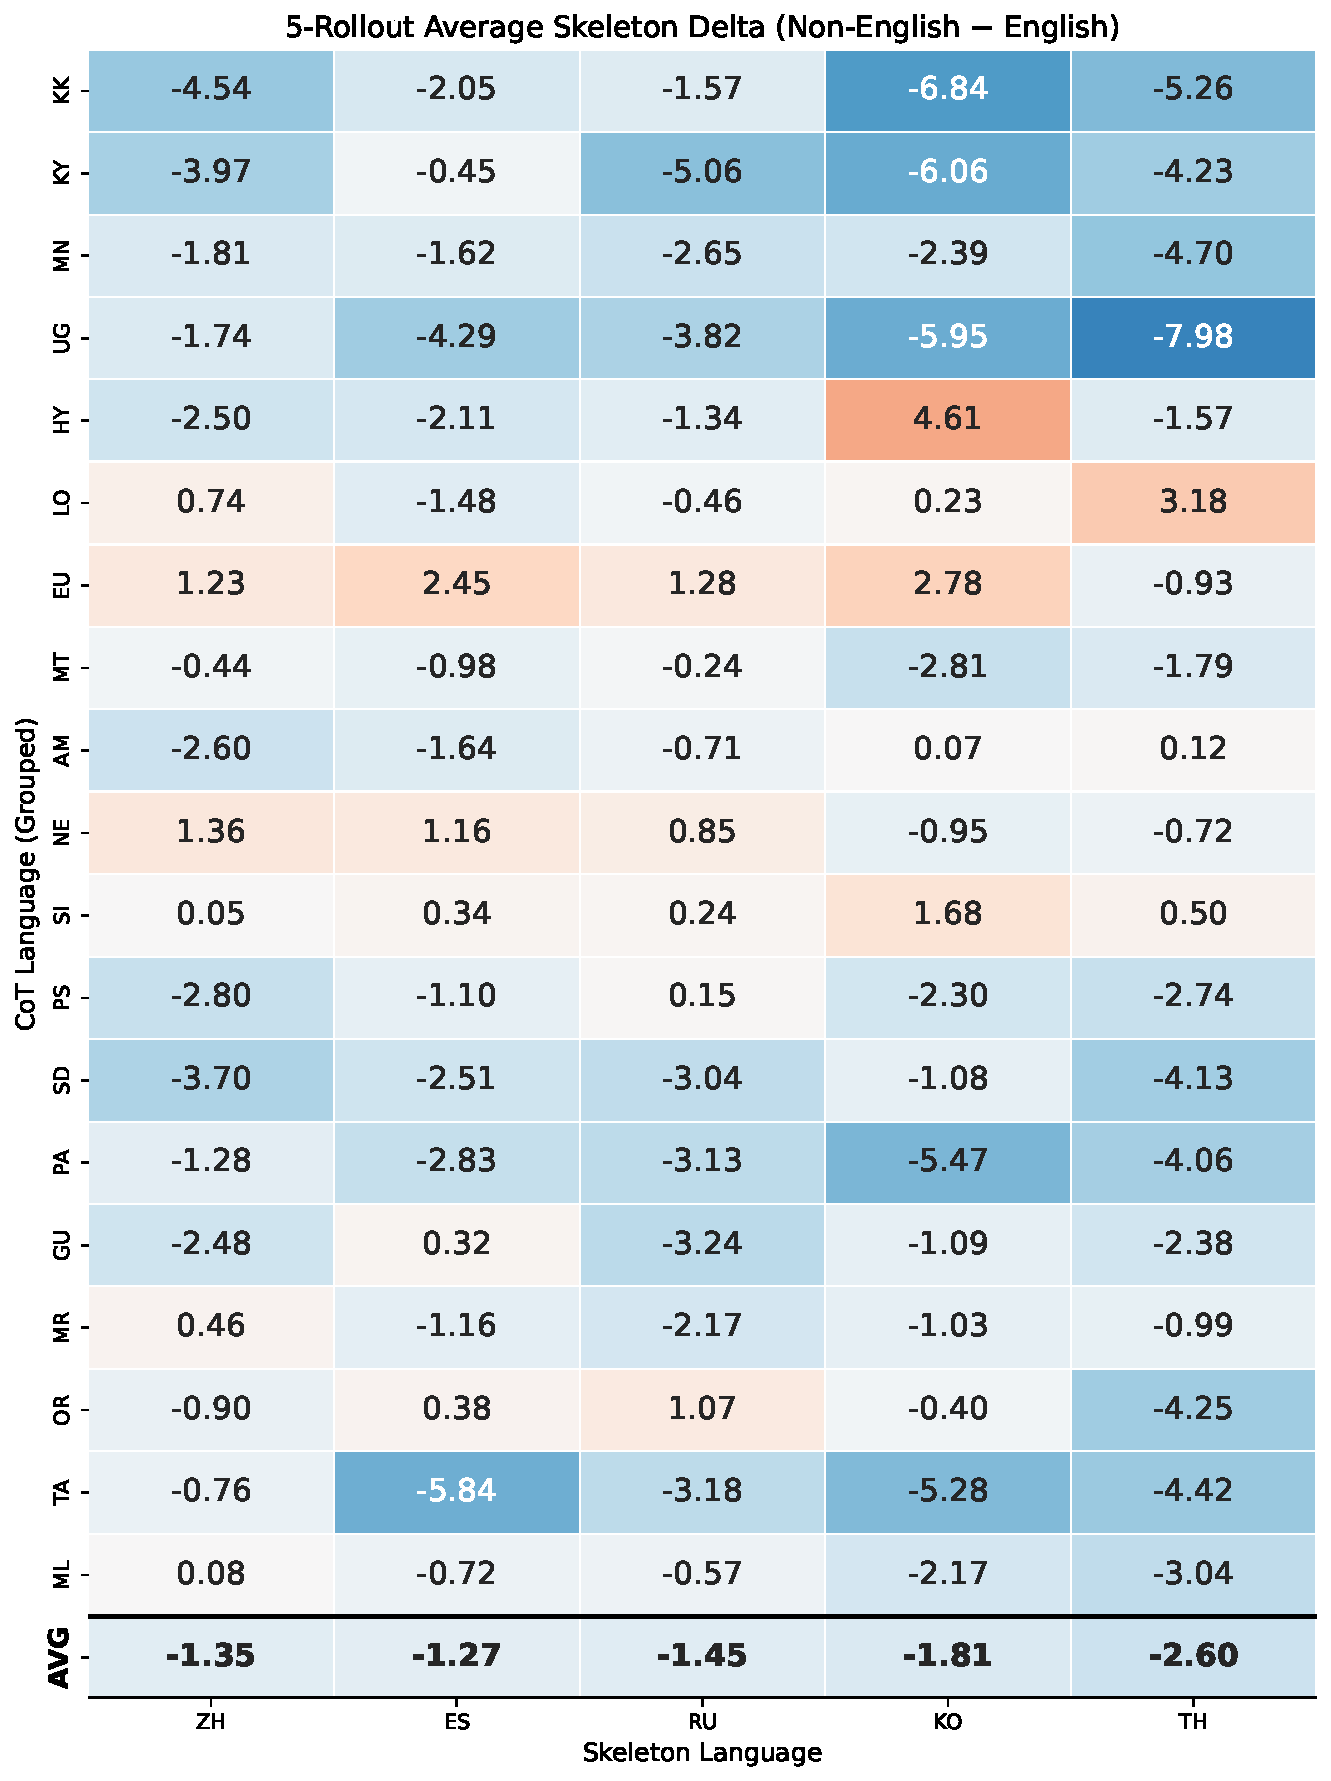
\includegraphics[width=\linewidth]{Figures/Images/5rollout.pdf}
        \caption{Multi-rollout ($T{=}0.7$, $N{=}5$)}
        \label{fig:heatmap-rollout5}
    \end{subfigure}
    \caption{\small Performance differences (Non-English $-$ English) on MGSM under CoT-$\ell_t$ with \textsc{Qwen2.5-7B}. The English skeleton is replaced with five Non-English skeletons (ZH, ES, RU, KO, TH); the same skeleton set is used in both panels. \textbf{(a)} Greedy decoding (single rollout). \textbf{(b)} Multi-rollout sampling ($T{=}0.7$, $N{=}5$).}
    \label{fig:cross-lingual-skeleton}
    \vspace{-0.15in}
\end{figure*}
\paragraph{General Trends: English as a Stable Anchor.}
Fig.~\ref{fig:cross-lingual-skeleton} presents the performance differences (Non-English − English) under the CoT-$\ell_t$ setting using \textsc{Qwen2.5-7B}, where the English skeleton is replaced with five non-English skeletons (Chinese, Spanish, Russian, Korean, and Thai). From an overall perspective, uniformly applying non-English skeletons instead of English leads to a decrease in average performance across languages, ranging from 0.56 to 2.32 points. These results reaffirm that English functions as the most general and stable reasoning skeleton for the majority of languages. However, when examining individual languages, particularly those for which English skeletons had shown negative effects, notable exceptions emerge.
% Figure~\ref{fig:cross-lingual-skeleton} presents the performance differences (Non-English −- English) under the CoT-$\ell_t$ setting using \textsc{Qwen2.5-7B}, where the English skeleton is replaced with five non-English skeletons (Chinese, Spanish, Russian, Korean, and Thai). Overall, replacing English with non-English skeletons decreases average performance by 0.56 to 2.32 points, reaffirming English as the most stable reasoning skeleton. However, for languages where English skeletons had shown negative effects, notable exceptions emerge.


\paragraph{Linguistic Affinity and Unexpected Gains.}
As shown in Tab.~\ref{tab:low-resource-mgsm}, languages that experienced performance degradation when using English skeletons often exhibit notable improvements when paired with skeletons from specific languages that share linguistic roots or grammatical structures. A representative example is Lao~(lo). While Lao suffers a performance drop when using an English skeleton ($-2.03$), its performance improves by 2.81 points when a Thai~(th) skeleton is used instead. We hypothesize that the high degree of grammatical and lexical similarity within the Tai–Kadai language family helps minimize information loss during translation and facilitates more direct knowledge transfer. Similarly, Basque~(eu), a language isolate, shows a slight performance decrease with English skeletons ($-0.84$), but gains a substantial +6.32 improvement when paired with a Korean~(ko) skeleton, which is also agglutinative and shares an SOV word order. This observation suggests that structural alignment may positively contribute to the coherence of the reasoning process. A particularly noteworthy case is Maltese~(mt). Although Maltese experiences the largest performance drop when using English skeletons ($-5.65$), it shows a +6.60 improvement with a Spanish~(es) skeleton, reflecting its Romance language influences. Interestingly, an even larger gain of +9.05 is observed with a Russian~(ru) skeleton, despite the significant linguistic distance between the two languages. This finding indicates that the transfer effects of skeletons may arise from a complex interplay of factors that cannot be fully explained by linguistic similarity alone.

\paragraph{Linguistic Affinity is Not Enough.}
In contrast, we also observe that neither geographic proximity nor shared writing systems necessarily guarantees positive transfer. Mongolian (mn), despite sharing the Cyrillic script, exhibits a performance drop of $-5.53$ when using Russian skeletons, which stands in stark contrast to the positive effects observed for Kazakh (kk) and Kyrgyz (ky) with Russian skeletons. Similarly, Uyghur (ug) shows a decrease of $-6.45$ when paired with a geographically proximate Chinese skeleton. These contrasting results suggest that surface-level similarities alone are insufficient, and that additional latent factors such as the co-occurrence frequency of the two languages within pretraining data and the absolute amount of available data should be jointly considered.

\paragraph{The Necessity of LASEF.}
In conclusion, while English is clearly the most powerful general solution, the results in Tab.~\ref{tab:low-resource-mgsm} and Fig.~\ref{fig:cross-lingual-skeleton} indicate that it is not the only viable answer. In particular, in settings where English skeletons fail to be effective, alternative skeleton languages that exhibit higher compatibility with the target language or are better aligned in structural terms can play a crucial role in enabling performance recovery. This suggests that the choice of skeleton language is not a fixed rule, but rather a core design variable that should be adaptively optimized according to the characteristics of the target language and the model’s data distribution. Consequently, the necessity of systematically exploring such optimal combinations through \LASEF becomes even more pronounced.